% =============================================================================
% Pesquisa com clientes e usuarios: entrevistas individuais e survey
% (projeto Riachuelo, PRO3474).
%
% Substitui 6b-planejamento_entrevistas_individuais.tex. Mudancas principais:
%   - remove a definicao formal do problema (tres elementos); a definicao do
%     problema tera secao propria, apos a analise de mercado, em etapa futura
%     do relatorio.
%   - o roteiro completo das entrevistas passa para o Anexo A
%     (3-pos/3-anexo-roteiro-entrevistas.tex); o corpo desta secao discute o
%     racional metodologico, nao as perguntas uma a uma.
%   - inclui uma discussao do survey quantitativo, com placeholders de
%     imagem para os prints do formulario (a inserir pelo autor).
%
% Gaps sinalizados no texto (nao preenchidos com conteudo inventado):
%   - a divergencia entre a segmentacao estrutural (Premium/Popular) e
%     eventuais clusters comportamentais obtidos por outras analises
%     quantitativas do projeto ainda nao foi avaliada.
%   - nenhuma imagem do formulario de survey foi incluida: os prints ainda
%     serao capturados pelo autor (ver placeholders na Seção~\ref{subsec:survey}).
% =============================================================================

\section{Planejamento de pesquisa}
\label{sec:pesquisa_clientes_usuarios}

A caracterização de clientes e usuários da Seção~\ref{sec:clientes_usuarios} deixou perguntas em aberto sobre comportamento, necessidades e diferenças entre Cliente Premium e Cliente Popular. Esta seção documenta duas frentes de pesquisa conduzidas para reduzir essas lacunas: entrevistas individuais semiestruturadas e um survey quantitativo. As duas frentes investigam as mesmas hipóteses (Seção~\ref{subsec:clientes_lacunas}) por caminhos diferentes e complementares.

\subsection{Entrevistas individuais semiestruturadas}
\label{subsec:entrevistas}

A equipe optou por entrevistas individuais, em vez de outros formatos qualitativos, por quatro razões.

\begin{enumerate}
    \item As fricções de compra tocam em restrição de orçamento, dependência do vendedor e insegurança sobre a própria capacidade de decidir sozinho. Um entrevistado tende a suavizar esses temas diante de outras pessoas.
    \item A reconstrução detalhada de uma jornada de compra exige que o entrevistador volte a um ponto do relato quantas vezes for necessário, o que depende de tempo dedicado a uma única pessoa.
    \item Contradições entre o que a pessoa diz preferir e o que relata ter feito na prática constituem um dos principais tipos de dado que esta pesquisa busca capturar. O entrevistador confronta essas contradições com mais clareza numa conversa a sós.
    \item A comparação entre Cliente Premium e Cliente Popular fica mais limpa quando cada entrevista segue o mesmo roteiro de forma independente, sem a influência da composição de um grupo específico sobre o que emerge na conversa.
\end{enumerate}

As entrevistas buscam entender o comportamento real do consumidor na loja física: como ele busca, escolhe, experimenta e paga por um produto, e onde aparecem fricção, dependência de atendimento e desconfiança. A investigação parte da experiência do entrevistado, não de uma solução já em estudo, e permite que necessidades ainda não identificadas pelo projeto apareçam de forma espontânea.

A seleção de entrevistados usou a mesma segmentação estrutural da Seção~\ref{subsec:segmentacao_clientes_usuarios}: Cliente Premium, recrutado a partir de lojas ou formatos voltados a público de maior poder aquisitivo, e Cliente Popular, recrutado a partir do varejo de massa. O critério de classificação é o formato da loja frequentada. A equipe planejou de 8 a 12 entrevistas, com paradas para análise a cada 4 ou 5 entrevistas; se os temas relatados começarem a se repetir sem produzir informação nova, o número final pode ser menor. Cada entrevista durou entre 20 e 30 minutos, com participantes que compraram roupa em loja física nos últimos três meses.

O roteiro percorre, nesta ordem, a reconstrução de uma jornada de compra recente, a busca e a disponibilidade de produto, a autonomia em relação ao vendedor, a fila e o pagamento, a confiança em processos sem checagem humana, e um espaço aberto para necessidades não previstas. Ao final, de forma condicional, o roteiro apresenta uma hipótese de solução em estudo pela equipe, para testar percepção de valor, barreiras e objeções, sem assumir que ela resolve o problema do consumidor. O Anexo~\ref{anexo:roteiro_entrevistas} documenta o instrumento completo, com todas as perguntas na ordem em que são feitas.


\subsection{Survey quantitativo}
\label{subsec:survey}

O survey complementa as entrevistas com alcance maior: mede a frequência e a relevância declarada de cada fricção numa amostra maior de consumidores, e permite comparar Cliente Premium e Cliente Popular por meio de afirmações padronizadas. O objetivo desta etapa é caracterizar os dois grupos, nenhuma afirmação do instrumento pergunta diretamente se o consumidor gostaria da trava antifurto conectada ao aplicativo.

O instrumento usa afirmações avaliadas em escala de concordância (1, discordo totalmente, a 5, concordo totalmente) e perguntas de frequência (nunca, raramente, às vezes, frequentemente, sempre). Cada afirmação está amarrada a uma hipótese específica da Seção~\ref{subsec:clientes_lacunas}, sem perguntas incluídas por curiosidade. Para maiores detalhes, disponibilizamos o link para avaliação: \url{https://forms.gle/Qv1ENMtbyjQpuH798}

A primeira pergunta do survey identifica a unidade da Riachuelo que o respondente frequenta com maior frequência. A equipe classifica cada unidade informada como Premium ou Popular a partir de um mapeamento prévio (perfil de shopping ou região, ticket médio da loja), feito antes da aplicação. O respondente não se autodeclara premium ou popular; a classificação entra na análise depois da coleta.

\begin{figure}[H]
    \centering
    \caption{Pergunta de qualificação do survey}
    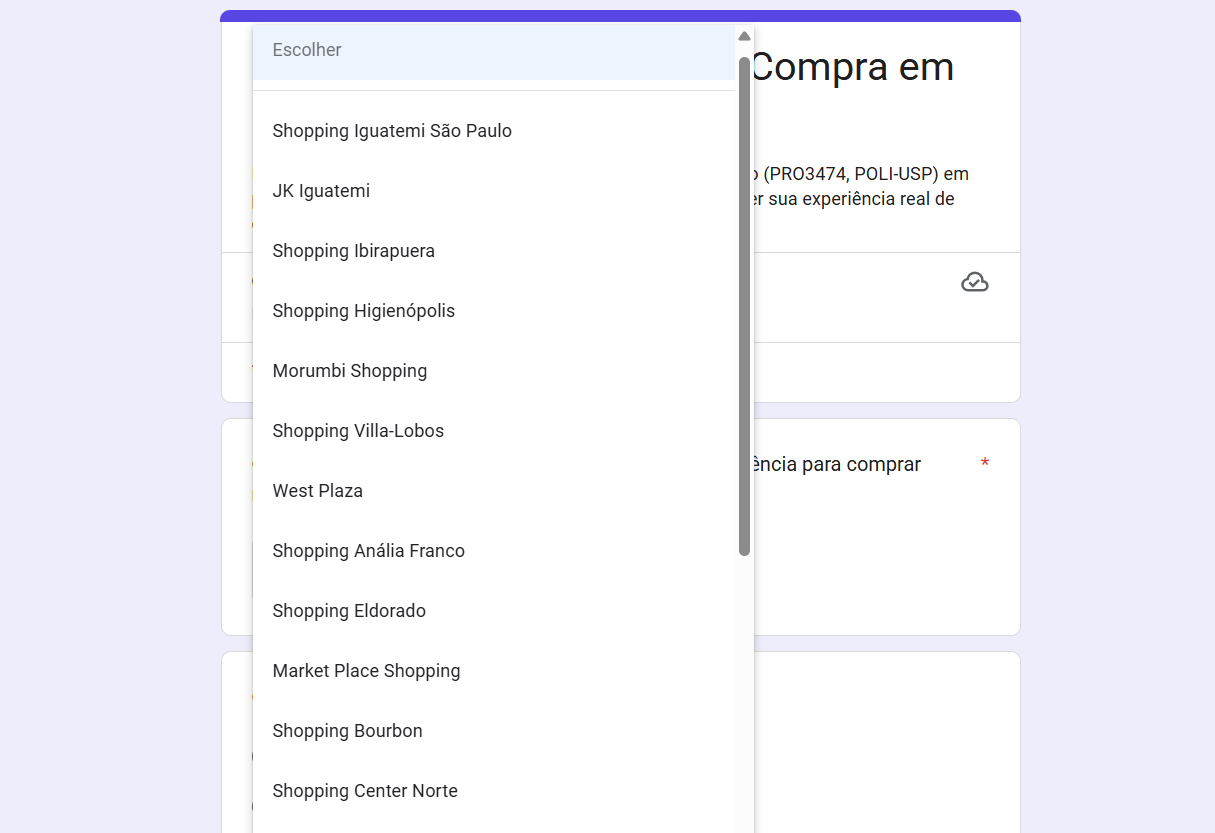
\includegraphics[width=0.5\textwidth]{imagens/pesquisa/shoppings.png}
    \label{fig:survey-qualificacao}
    \source{Autoria própria}
\end{figure}

\textbf{Aspectos investigados:} o instrumento cobre cinco dimensões, cada uma amarrada a uma das hipóteses da Seção~\ref{subsec:clientes_lacunas}: disponibilidade e facilidade de encontrar produtos; atendimento e autonomia, segmentados por momento da jornada (escolha, prova, pagamento); fila e tempo de pagamento; confiança em tecnologia e uso de canais digitais; e segurança e confiança no processo de saída da loja.

\begin{figure}[H]
    \centering
    \caption{Exemplo de bloco de afirmações em escala de concordância}
    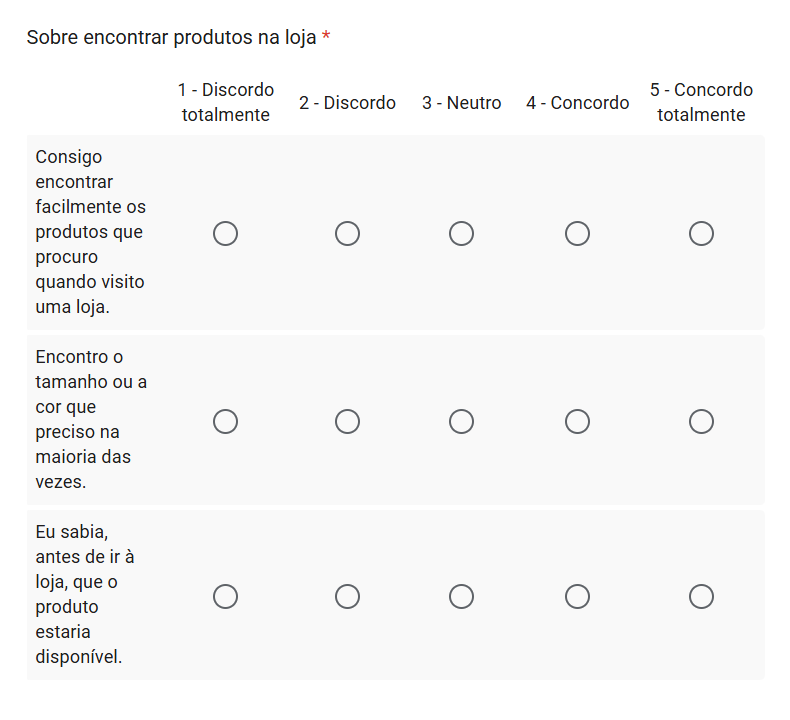
\includegraphics[width=0.5\textwidth]{imagens/pesquisa/likert.png}
    \label{fig:survey-bloco-concordancia}
    \source{Autoria própria}
\end{figure}

\begin{figure}[H]
    \centering
    \caption{Exemplo de pergunta de frequência}
    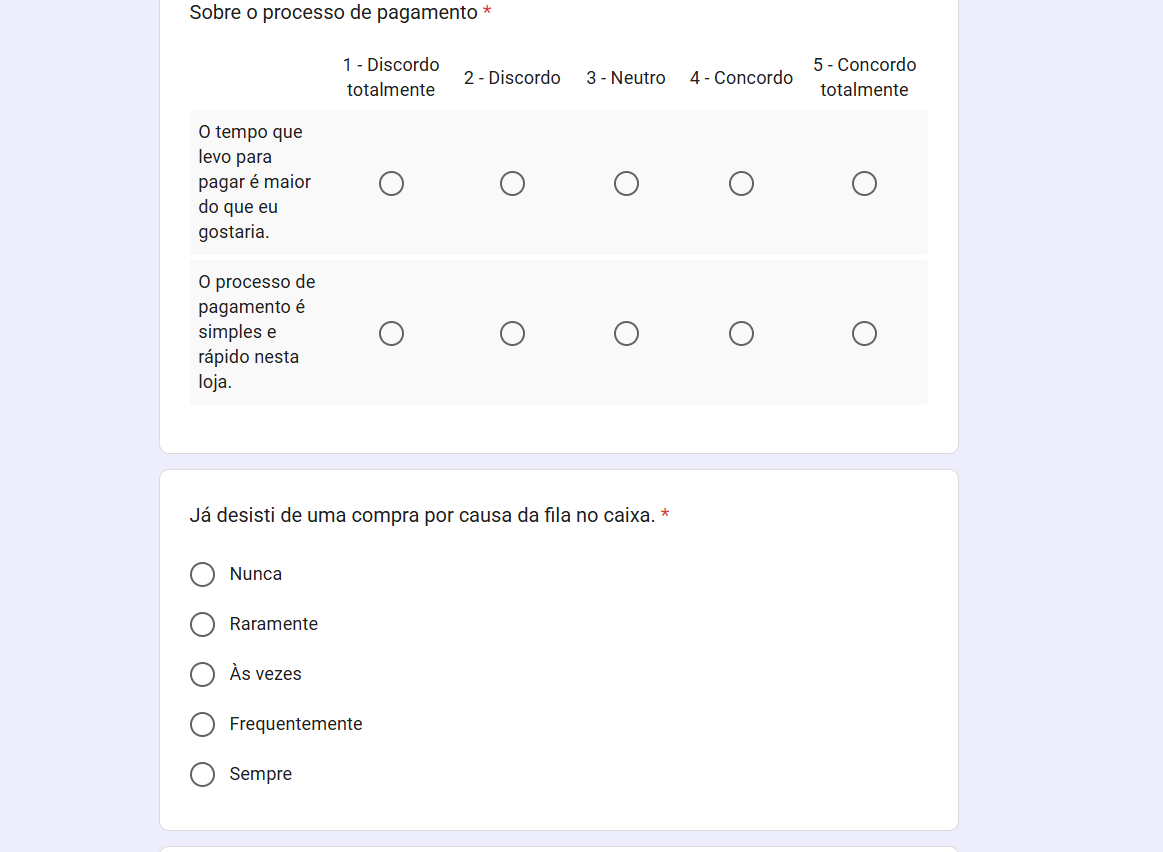
\includegraphics[width=0.5\textwidth]{imagens/pesquisa/desistencia.png}
    \label{fig:survey-pergunta-frequencia}
    \source{Autoria própria}
\end{figure}

O survey mede quantas pessoas relatam cada fricção e com que intensidade. As entrevistas explicam por que essas fricções ocorrem e em que contexto. Nenhuma das duas frentes isolada responde às duas perguntas ao mesmo tempo, e por isso a equipe as conduz em paralelo.

A classificação por unidade frequentada assume que cada loja tem um perfil predominante único. Isso falha em dois casos: um respondente frequenta mais de uma unidade com perfis diferentes, ou uma unidade tem público misto, como uma loja de rua em bairro de alta renda. O instrumento também depende de autorrelato, sujeito aos mesmos vieses de qualquer survey de autopercepção: um respondente pode subestimar comportamentos que julga socialmente indesejáveis, como depender do vendedor para decidir uma compra.
